\section{Upgrade-Info CUBE Project Assistant} % Major section
% Example citation \cite{Figueredo:2009dg}. (Literaturangabe; Literaturliste)

Ihre CUBE Project Assistant-Instanz wird auf die Version 2.12 aktualisiert. Wir führen neue Funktionen ein. Gleichzeitig werden einige Funktionen angepasst. Um den Umstieg reibungslos zu gestalten, sind die wichtigsten Änderungen untenstehend beschrieben.

\subsection{Dokumente hochladen}
In verschiedenen Modulen können nicht nur Dokumente verknüpft, sondern neue Dokumente hochgeladen werden. Zum einen wird damit die Dokumentenverknüpfung (z.B. Sitzungsbeilage) erstellt, zum anderen steht das hochgeladen Dokument in der Dokumentenablage ebenfalls zur Verfügung.

\begin{figure}[H]
\center{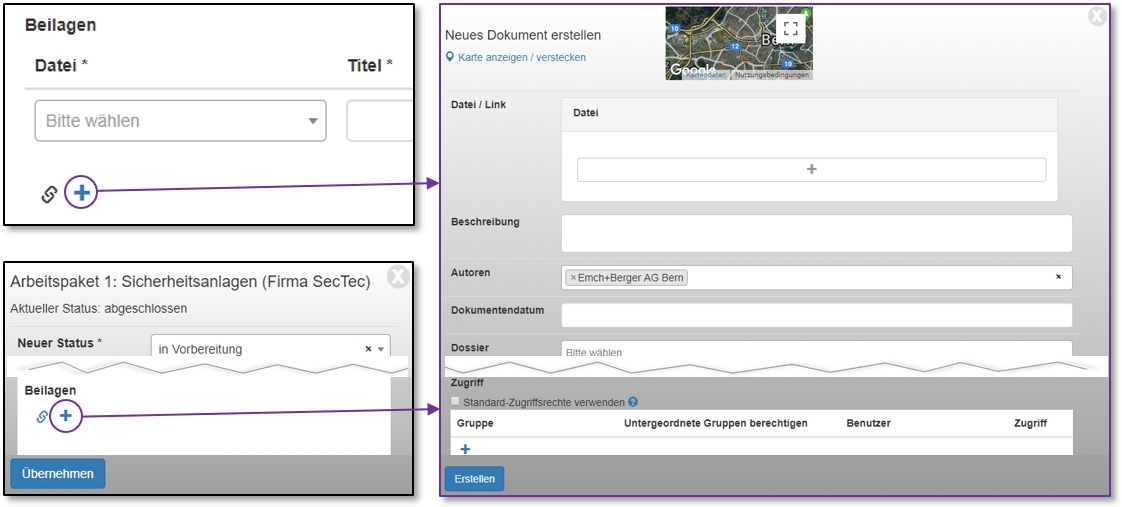
\includegraphics[width=1\linewidth]{../chapters/01_generisch/pictures/FileUpload.jpg}}
% \caption{Neue Sitzung erfassen}
% \label{fig:speciation}
\end{figure}

Klicken Sie jeweils auf das Pluszeichen 
\includegraphics[height=12pt]{/Icons/Pluszeichen.jpg}, wird ein zusätzliches Fenster geöffnet. Wie in der Dokumentenablage lassen sich nun weitere Angaben zum Dokument hinzufügen.

\subsection{Dokumente per Link versenden}
Dokumente können in Emails als Attachement oder mit sicherem Link versendet werden.

\begin{figure}[H]
\center{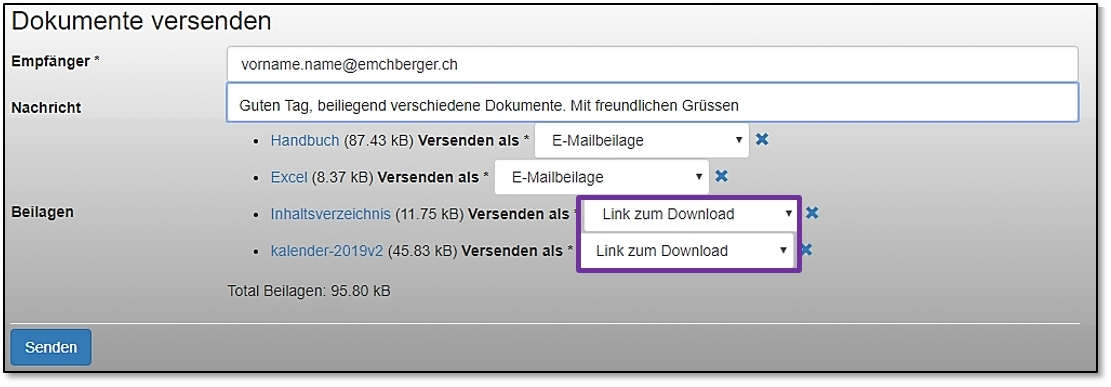
\includegraphics[width=1\linewidth]{../chapters/01_generisch/pictures/EmailLink.jpg}}
% \caption{Neue Sitzung erfassen}
% \label{fig:speciation}
\end{figure}

Bei der Auswahl 'Link zum Download' wird eine sichere Verbindung zu CUBE PA erstellt. Der Empfänger muss sich für das Herunterladen des Dokuments bei CUBE PA nicht anmelden. Dieser sichere 'Link' hat eine Gültigkeitsdauer von 30 Tagen und läuft danach automatisch ab.

\subsection{Datensätze in der Übersicht bearbeiten}
In der Adressliste wie auch in den Pendenzen können die gewünschten Änderungen gerade in der Übersicht vorgenommen werden:

\begin{figure}[H]
\center{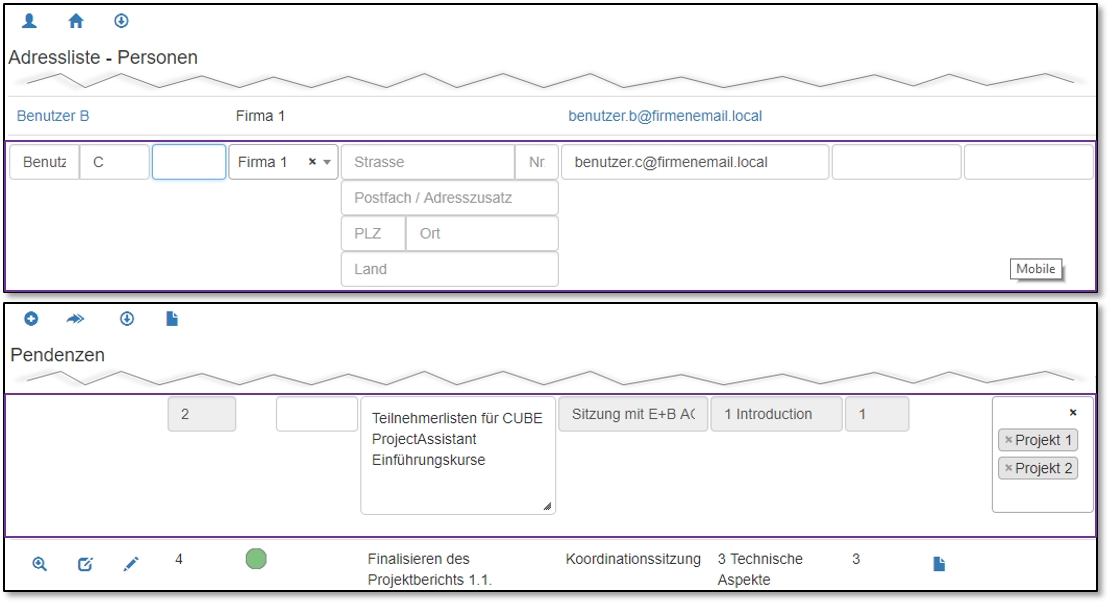
\includegraphics[width=1\linewidth]{../chapters/01_generisch/pictures/InlineEdit.jpg}}
% \caption{Neue Sitzung erfassen}
% \label{fig:speciation}
\end{figure}

\textbf{Einige Features:}
\begin{compactitem}
	\item Mit Doppelklick in einen Datensatz wird dieser für die Bearbeitung geöffnet
	\item Erneuter Doppelklick speichert die Daten und schliesst die Bearbeitung
	\item Ist bereits ein Datensatz für die Bearbeitung geöffnet, kann kein zweiter geöffnet werden (Meldung erscheint)
	\item Ist eine Geschäftsadresse hinterlegt, wird diese mit entsprechendem Vermerk angezeigt. Wird eine separate Adresse hinterlegt, hat diese Priorität - wird sie wieder gelöscht, erscheint erneut die Geschäftsadresse
	\item Mit Klick auf den Stift erreichen Sie die gleiche Funktion wie mit Doppelklick in den Datensatz
	\item Sie können mit Klick auf das Bearbeitungssymbol 
\includegraphics[height=12pt]{/Icons/Bearbeiten.jpg} auch die Formularseite öffnen und Änderungen vornehmen.
\end{compactitem}

\vspace{\baselineskip}

\textbf{Tipp:} Neu haben Sie jeweils oben in der Bildmitte zwei Schaltflächen: 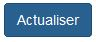
\includegraphics[height=14pt]{/Icons/B_Uebernehmen.jpg} und 
\includegraphics[height=14pt]{/Icons/ueb_schliessen.png}. Mit Klick auf 
\includegraphics[height=14pt]{/Icons/ueb_schliessen.png} gelangen Sie in der Regel auf die Übersichtsseite.

\vspace{\baselineskip}

Auf YouTube finden Sie verschiedene Tutorial-Videos, welche Ihnen weitere hilfreiche Unterstützung für die Arbeit mit CUBE Project Assistant bieten \href{https://www.youtube.com/channel/UCYWA8nERo4vTPYWP0WJ32hw}{\color{blue}[Link]}.

\vspace{\baselineskip}

Die Detailbeschreibungen zu obigen Funktionen finden Sie im CUBE PA-Benutzerhandbuch. Für weitere Fragen kontaktieren Sie uns unter {\color{red} cube.support@emchberger.ch}.
